% Switch between de/en and ids/tks as needed
\documentclass[de,ids]{fziartcl}
% \documentclass[en,tks]{fziartcl}
% \documentclass[de,ids]{fziartcl}
% \documentclass[en,ids]{fziartcl}

\include{preamble}

% Place your name here
\author{Dennis Nienhüser}

% You can override the date, if needed
% \date{21.11.2012}

\title{Eine beispielhafte Studie}

\begin{document}

\maketitle

\tableofcontents
\newpage

\section{Einleitung}
\blindtext

\begin{figure}[h]

\begin{minipage}{.5\textwidth}
\centering

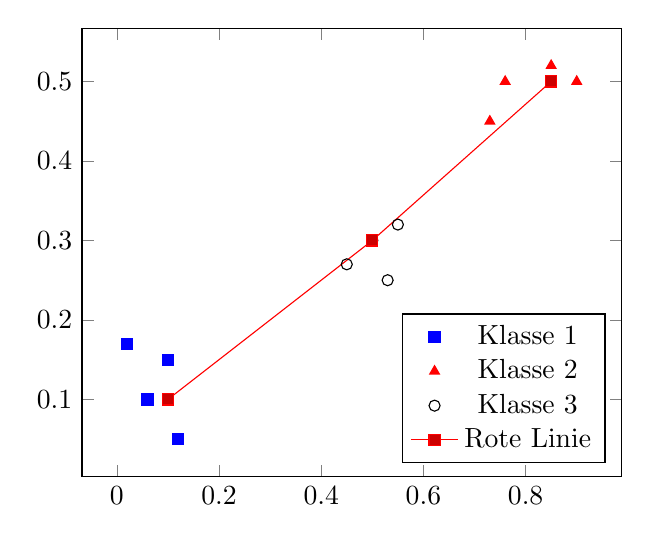
\begin{tikzpicture}
\begin{axis}[scatter/classes={
        a={mark=square*,blue},%
        b={mark=triangle*,red},%
        c={mark=o,draw=black}},
        legend pos=south east]

        \addplot[scatter,only marks,
                scatter src=explicit symbolic]
                coordinates {
                        (0.1,0.15)  [a]
                        (0.45,0.27) [c]
                        (0.02,0.17) [a]
                        (0.06,0.1)  [a]
                        (0.9,0.5)   [b]
                        (0.5,0.3)   [c]
                        (0.85,0.52) [b]
                        (0.12,0.05) [a]
                        (0.73,0.45) [b]
                        (0.53,0.25) [c]
                        (0.76,0.5)  [b]
                        (0.55,0.32) [c]
                };
        \addplot coordinates
                {(0.1,0.1) (0.5,0.3) (0.85,0.5)};
        \legend{Klasse 1, Klasse 2, Klasse 3, Rote Linie}
\end{axis}
\end{tikzpicture}

\end{minipage}
\begin{minipage}{.5\textwidth}
\centering

\begin{tikzpicture}[
      start chain=1 going right,start chain=2 going below,node distance=-0.15mm
    ]
    \node [on chain=2] {Tape};
    \node [on chain=1] at (-1.5,-.4) {\ldots};
    \foreach \x in {1,2,...,11} {
        \x, \node [draw,on chain=1] {};
    }
    \node [name=r,on chain=1] {\ldots};
    \node [name=k, arrow box, draw,on chain=2,
        arrow box arrows={east:.25cm, west:0.25cm}] at (-0.335,-.65) {};
    \node at (2.0,-.85) {Read/write head};
    \node [on chain=2] {};
    \node [draw,on chain=2] {Program};
    \chainin (k) [join]; % Verbindung vom Programm zum Leseschreibkopf
\end{tikzpicture}

\end{minipage}

\captionsetup{singlelinecheck=off}
\caption[foo bar]{Das ist meine Grafik. Es gibt viele solcher Grafiken, aber diese gehört mir. Oder nicht?!
\begin{itemize}
 \item \url{http://www.texample.net/tikz/examples}
 \item \url{http://pgfplots.sourceforge.net/gallery.html}
\end{itemize}}
\end{figure}

\subsection{Robot Operating System}
Das Robot Operating System bietet Kommunikationsschnittstellen für ein verteiltes System in dem Knoten Nachrichten in sogenannten Topics veröffentlichen und Dienste anbieten können
\section{Lokalizierung der Roboter}
Die Lokalisierung unserer Roboter bietet entweder Gmapping ROS-Packet oder die Cartographer von Google.Wenn die Laufroboter die Selbstlokalisierung ausführt,wird erst die Ros-Launch file eingegeben dann die entsprechende Ros-Packet werden gleich aufgerufen.Folgendes wird über den Unterschied zwischen Gmapping und Google-Cartographer
diskutiert.

\subsection{Gmapping}
Kürzlich wurden Rao-Blackwellized Partikelfilter als effektive Mittel eingeführt, um das Problem der Simultanen Lokalisierung und Kartierung (SLAM) zu lösen. Dieser Ansatz verwendet einen Partikelfilter, in dem jedes Partikel eine individuelle Karte der Umgebung trägt. Eine zentrale Frage ist daher, wie die Anzahl der Partikel reduziert werden kann. Die Anzahl von Partikeln wird in einem Rao-Blackwell-Partikelfilter zum Erlernen von Gitterkarten reduziert. 
\\Einen Ansatz wird vorgeschlagen, um eine genaue Vorschlagsverteilung zu berechnen, die nicht nur die Bewegung des Roboters, sondern auch die jüngste Beobachtung berücksichtigt. Dies verringert die Unsicherheit über die Pose des Roboters im
Voraussage-Schritt des Filters drastisch. Darüber hinaus wird in Gmapping Algorithmus diese Ansatz verwendet, um selektiv Re-Sampling-Operationen durchzuführen,die das Problem der Partikelverarmung stark reduzieren.
\subsection{Cartographer}
Cartographer kann als zwei separate, aber verwandte Systeme gesehen werden. Der erste ist lokaler SLAM (manchmal auch Frontend genannt).Seine Aufgabe besteht darin, einen lokal konsistenten Satz von Submaps zu erstellen und sie miteinander zu verknüpfen, aber er wird sich im Laufe der Zeit verschieben. Die meisten Optionen befinden sich in "trajektory-builder-2d.lua" für 2D und "trajektory-builder-3d.lua" für 3D.
\\Das andere System ist ein globales SLAM (manchmal als Backend bezeichnet). Es läuft in Hintergrundthreads und seine Hauptaufgabe besteht darin, Loop-Close-Constraints zu finden. Dies geschieht durch Scan-Matching-Scans gegen Submaps. Es enthält auch andere Sensordaten, um eine Ansicht auf höherer Ebene zu erhalten und die konsistenteste globale Lösung zu identifizieren. In 3D versucht es auch, die Richtung der Schwerkraft zu finden. Die meisten Optionen finden Sie in pose-graph.lua.
\\Bei einer höheren Abstraktion besteht die Aufgabe des lokalen SLAM darin, gute Submaps zu erzeugen, und die Aufgabe des globalen SLAM besteht darin, sie am konsequentesten zu verknüpfen.





\cite{quigley2009ros}.

\bibliography{example}

\end{document}
